\section{Light} \label{sec:Light}
	\begin{definition}[Photon]
		A \emph{photon} is an electric field (wave) propagating through another electric field.
	\end{definition}
The various $\theta$ used in Equations~\eqref{eq:Reflected Light},~\eqref{eq:Refracted Light} are measured from the surface normal.

\emph{Chromatic Dispersion} is the breaking up of polychromatic light by spectra.
Think of Pink Floyd's \textit{Dark Side of the Moon} album cover.
This happens because shorter wavelength, higher frequency light has a slightly higher index of refraction.
%	\begin{figure}[h!]
%		\centering
%		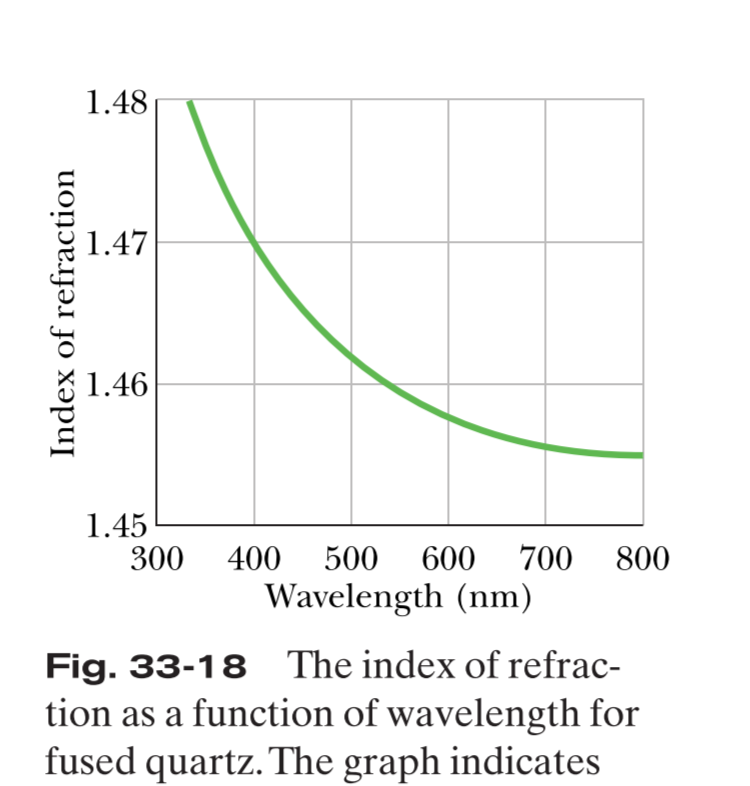
\includegraphics[scale=0.5]{Polychromatic_Light_Indices_Refraction.png}
%		\caption{Indices of Refraction for Polychromatic Light}
%		\label{fig:Indices of Refraction for Polychromatic Light}
%	\end{figure}

	\subsection*{Reflection} \label{subsec:Reflection}
		\begin{equation} \label{eq:Reflected Light}
			\theta_{reflected} = \theta_{incident}
		\end{equation}
		
	\subsection*{Refraction} \label{subsec:Refraction}
		\begin{definition}[Snell's Law] \label{def:Snell's Law}
			\begin{equation} \label{eq:Refracted Light} 
				n_{refract} \sin \left( \theta_{refract} \right) = n_{incident} \sin \left( \theta_{incident} \right)
			\end{equation}
		\end{definition}
		\begin{definition}[Index of Refraction] \label{def:Index of Refraction}
			\begin{equation} \label{eq:Index of Refraction}
				\begin{aligned}
					n_{i} &= \frac{c}{v_{i}} \\
					\lambda &= \frac{\lambda_{0}}{n} \\
				\end{aligned}
			\end{equation}
		\end{definition}
	
	\subsection*{Total Internal Reflection} \label{subsec:Total Internal Reflection}
		\begin{definition}[Total Internal Reflection] \label{def:Total Internal Reflection}
			Total Internal Reflection occurs when the \emph{refracted light's angle is $\frac{\pi}{2}$}.
			\begin{equation} \label{eq:Total Internal Reflection}
				n_{refract} \sin \left( \theta_{refract} \right) = n_{incident} \sin \left( \theta_{incident} \right) \text{, where } \theta_{refract} = \frac{\pi}{2}
			\end{equation}
		\end{definition}
		
	\subsection*{Interference and Diffraction} \label{subsec:Interference and Diffraction}
		\begin{definition}[Huygen's Principle] \label{def:Huygen's Principle}
			Any point on a plane wavefront can be treated as a source of outgoing spherical waves.
			\begin{note}
				This is a mathematical construct/model.
			\end{note}
		\end{definition}
		\begin{definition}[Phase Difference] \label{def:Phase Difference}
			Waves from the same source, but measured in such a way that there is a Path Length Difference (PLD) between them will have a \emph{phase difference}.
			\begin{equation} \label{eq:Phase Difference}
				\varphi = \frac{2 \pi \PLD}{\lambda}
			\end{equation}
		\end{definition}
	All \nameref{subsec:Interference and Diffraction} equations used from here on out are based on Equation~\eqref{eq:Phase Difference}.
		\begin{definition}[Single Slit Diffraction] \label{def:Single Slit Diffraction}
			When waves propagate through a single slit, there is a Probability Distribution Function that describes where intensity of light is greatest and smallest.
			The location of the \emph{\textbf{minima}} are given in Equation~\eqref{eq:Minima of Single Slit Diffraction}
			\begin{equation} \label{eq:Minima of Single Slit Diffraction}
				m \lambda = a \sin \left( \theta_{m} \right)
			\end{equation}
			\begin{note}
				$m$ is the number of minima from the central major distribution of intensity.
				\begin{enumerate}[noitemsep, nolistsep]
					\item First minima means $m=1$
					\item Second minima means $m=2$
					\item etc.
				\end{enumerate}
			\end{note}
			Thus, the equation for the \nameref{eq:Phase Difference of Single Slit Diffraction} is given in Equation~\eqref{eq:Phase Difference of Single Slit Diffraction}.
			\begin{equation} \label{eq:Phase Difference of Single Slit Diffraction}
				\varphi_{\text{Single Slit}} = \frac{2 \pi}{\lambda} a \sin \left( \theta \right)
			\end{equation}
		\end{definition}
		\begin{definition}[Double Slit Diffraction] \label{def:Double Slit Diffraction}
			This is really interference.
			The \emph{\textbf{maxima}} of the interference is given in Equation.
			\begin{equation} \label{eq:Maxima of Double Slit Diffraction}
				n \lambda = d \sin \left( \theta_{n} \right)
			\end{equation}
			\begin{note}
				$n$ is the number of maxima from the central major distribution of intensity.
				\begin{enumerate}[noitemsep, nolistsep]
					\item First maxima means $n=1$
					\item Second maxima means $n=2$
					\item etc.
				\end{enumerate}
			\end{note}
			Thus, the equation for the \nameref{eq:Phase Difference of Double Slit Refraction} is given in Equation~\eqref{eq:Phase Difference of Double Slit Refraction}.
			\begin{equation} \label{eq:Phase Difference of Double Slit Refraction}
				\varphi_{\text{Double Slit}} = \frac{2 \pi}{\lambda} d \sin \left( \theta \right)
			\end{equation}
		\end{definition}